In this section we present the results for simplified template cross sections Stage 1.1, a measurement strategy detailed in the CERN Yellow Report 4 of the LHC-HXSWG~\cite{YR4}. The reduced stage 1.1 bins are measured in forms of signal strength modifier. Figure~\ref{fig:stage1p1_mu} shows the results. The covariance matrix of the fitted results are shown in Figure~\ref{fig:cov} 

%=======
\begin{figure}[!htb]
        \vspace*{0.3cm}
        \begin{center}
                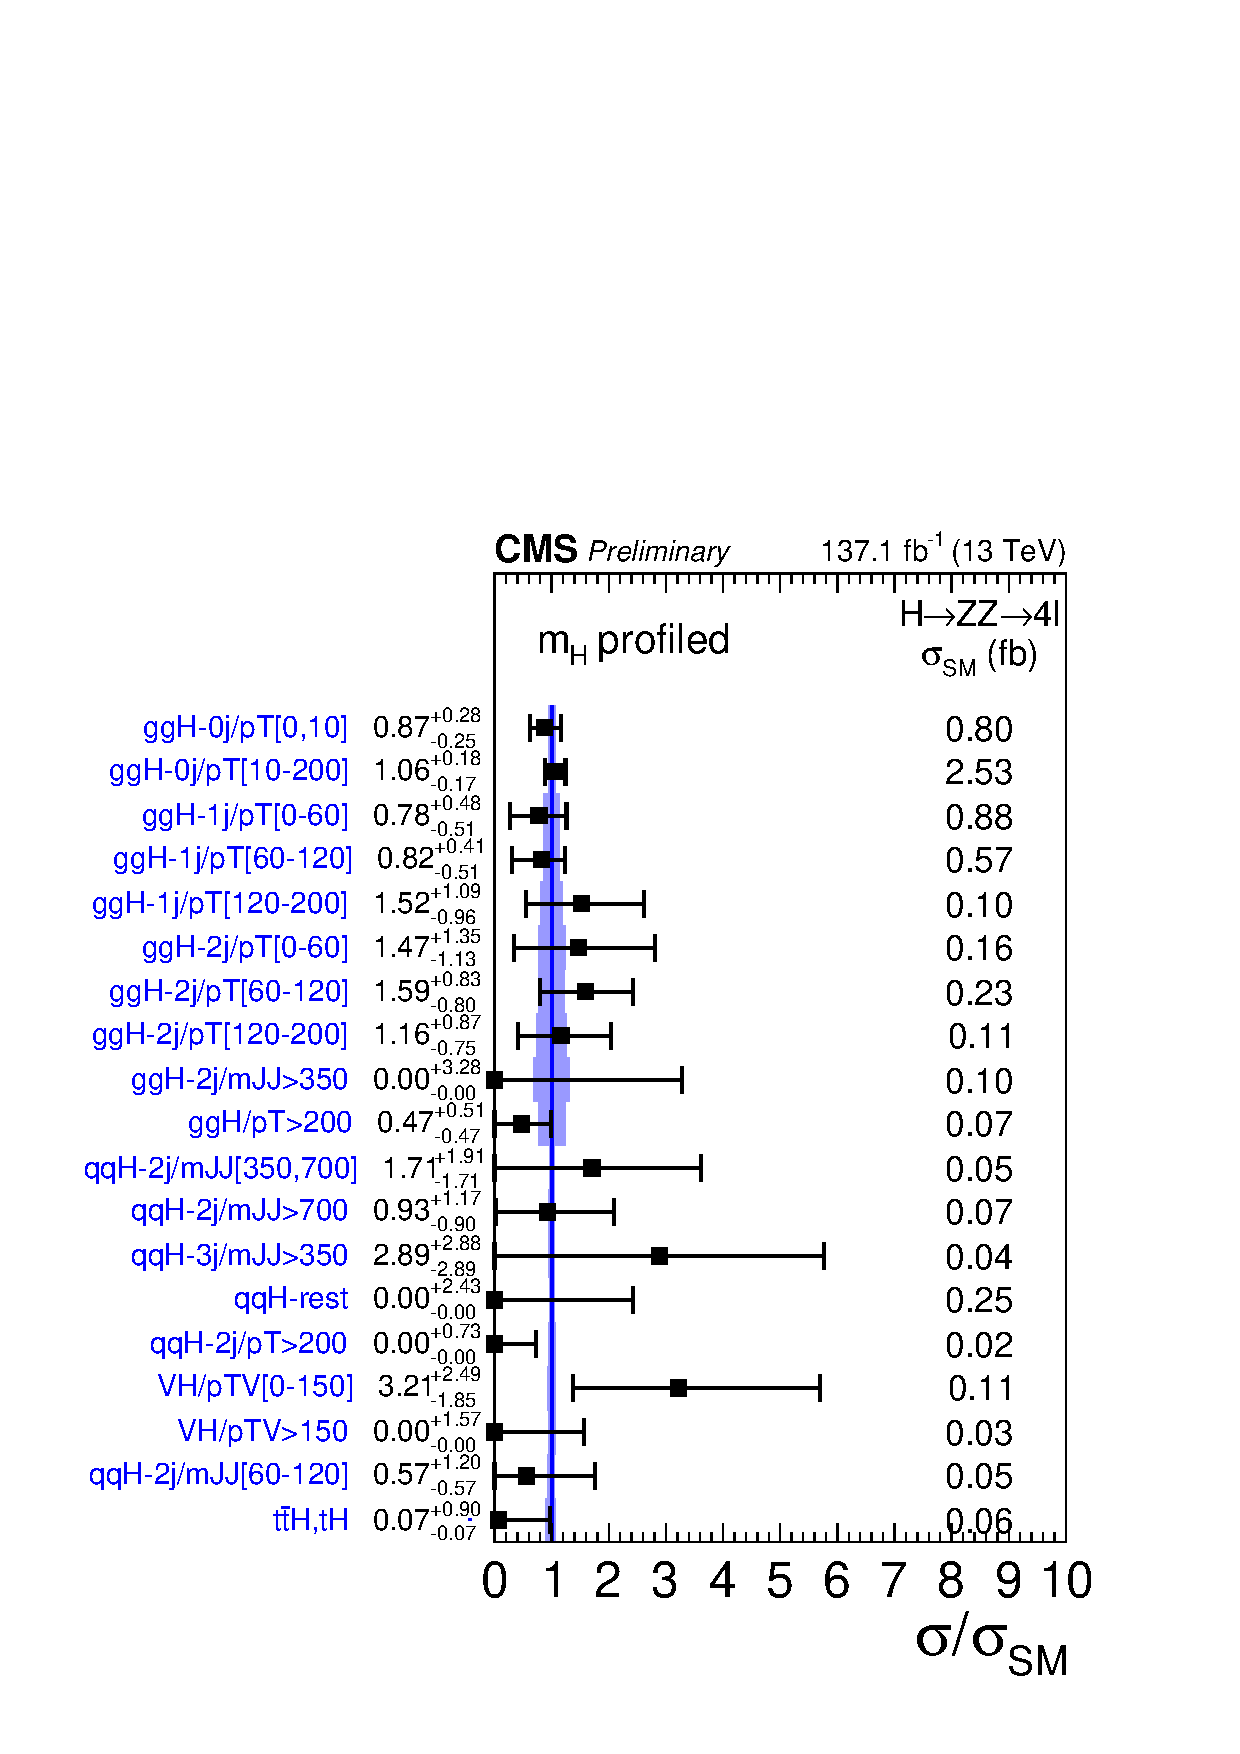
\includegraphics[width=0.8\textwidth]{Figures/results/stxs/mu_stage1_xsec.pdf}
                \caption{The ratios between measured cross sections and the SM prediction for stage1.1 bins, the \mH is profiled. The band around the vertical band shows the theoretical uncertainties on the SM cross section predictions for each stage 1.1 bin.}
                \label{fig:stage1p1_mu}}
        \end{center}
\end{figure}
%=======

%=======
\begin{figure}[!htb]
        \vspace*{0.3cm}
        \begin{center}
                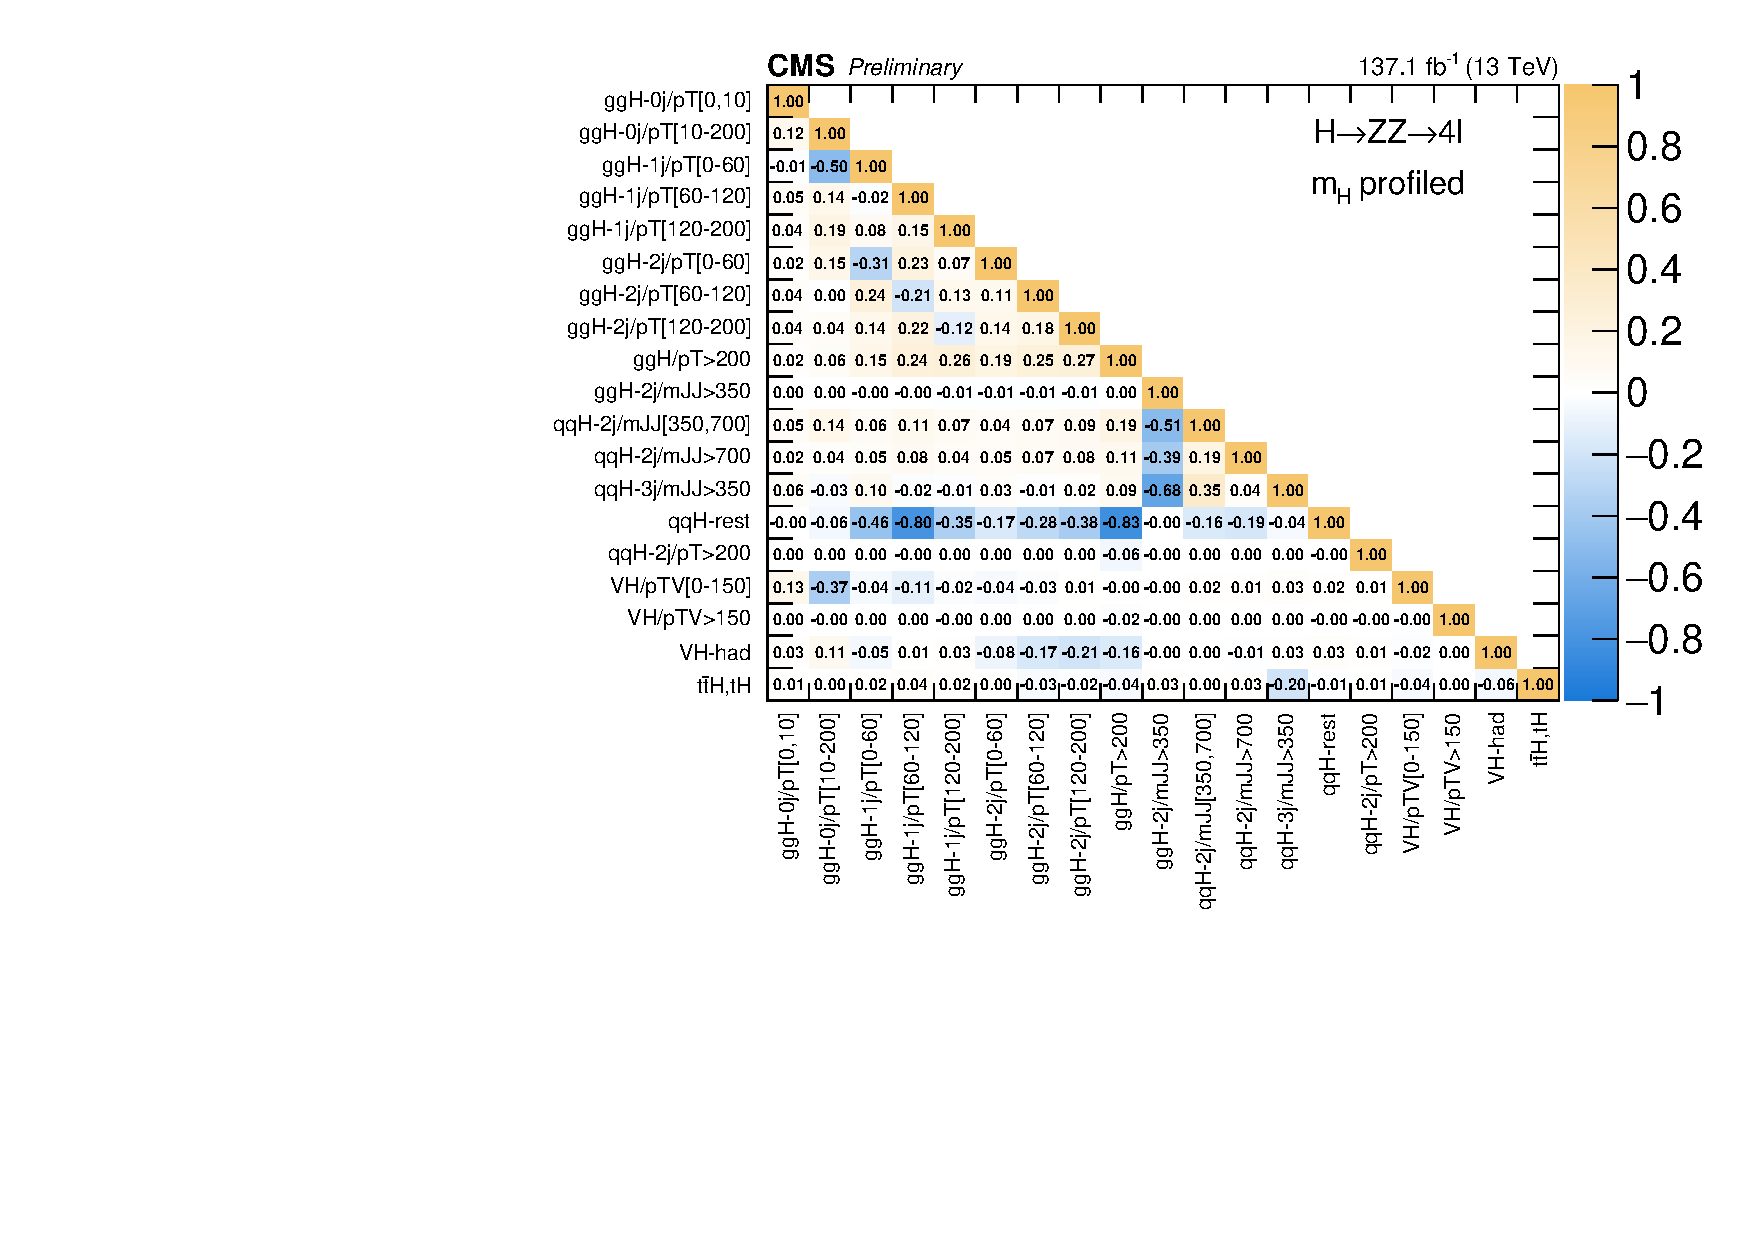
\includegraphics[width=0.8\textwidth]{Figures/results/stxs/scov_stage1.pdf}
                \caption{Covariance matrix of the fitted signal strength.}
                \label{fig:cov}}
        \end{center}
\end{figure}
%=======
